\documentclass{article}
\usepackage{graphicx}
\usepackage{amsmath}
\usepackage{parskip}
\usepackage[margin=1.5in]{geometry}
\title{Supporting Documentation for a Gyroscopic Fern}
\author{ijbd}
\begin{document}

	\section{Introduction}

	The goal of this iteration is to replace the stacked linear axes with a pair of rotating arms (figure \ref{fig:high-level-concept}). 
	This document serves as theoretical foundation and proof-of-concept for this idea.
	
	\begin{figure}[h!]
   		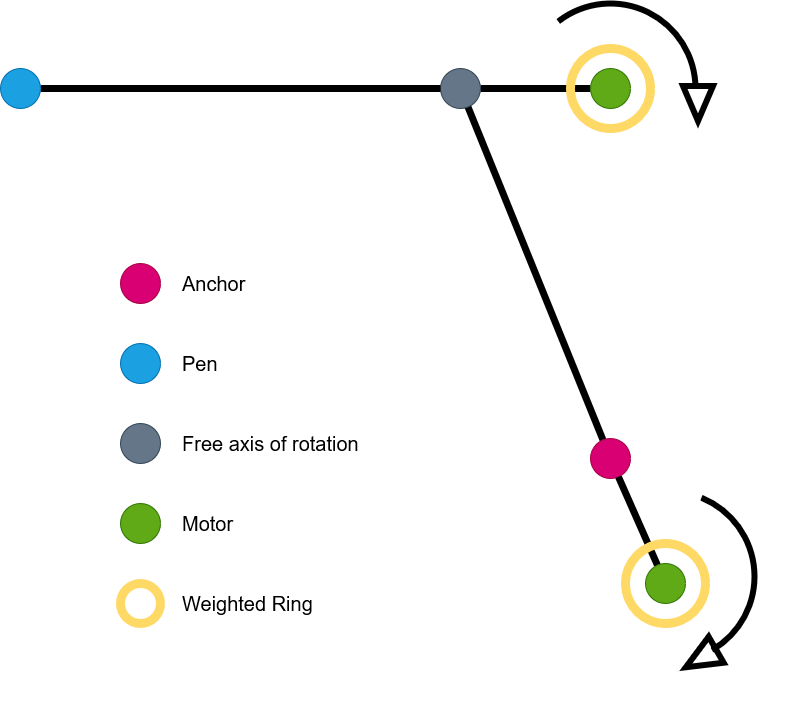
\includegraphics[width=\linewidth]{../diagrams/fern-v3-concept-diagram.png}   
		\caption{Birds-eye concept drawing of a gyroscopic fern.}
		\label{fig:high-level-concept}
	\end{figure}

	\section{Setup}

	To start, consider a single arm (figure \ref{fig:high-level-one-arm}). It has a motor on one end and an ambiguous mass on the other
	(e.g. a pen or another arm). 

	\begin{figure}[h!]
		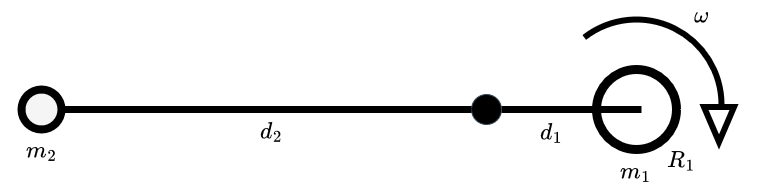
\includegraphics[width=\linewidth]{../diagrams/fern-v3-single-arm-diagram.png}   
	 	\caption{Body diagram for one arm.}
	 	\label{fig:high-level-one-arm}
 	\end{figure}

	Assume the motor and supporting rod are massless.
	With the system at rest, the angular momentum is zero. 
	Suppose the motor begins to spin such that the angular rotation about the rotor axis is $\omega$.
	We want to predict the resulting arm motion.
	The conservation of angular momentum says that the change in angular momentum of a system (lacking an external torques)
	is zero. 
	To express the rotational velocity of the arm as a function of motor speed,
	we can equate the angular momentum of the motor with the angular momentum of the arm.


	\section{Calculation}
	\subsection{Angular Momentum from the Spinning Ring}

	By definition...
	\begin{align}
		L &= \vec{r} \times\vec{p}
	 	&= \vec{r} \times m \vec{v} \\
		&= \int_m\vec{r}\times\vec{v} dm \\
		&= \int_{\theta}\vec{r}\times\rho\vec{v} d\theta
	\end{align}

	Where...
	\begin{align}
		\rho &= \frac{m_1}{2\pi}
	\end{align}

	The components of this integral are shown in figure \ref{fig:one-arm-integral}

	\begin{figure}[h!]
		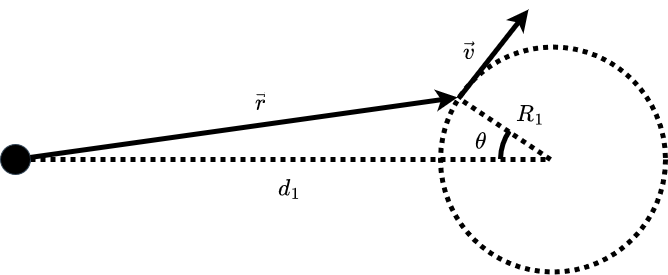
\includegraphics[width=\linewidth]{../diagrams/fern-v3-single-arm-integral-diagram.png}   
	 	\caption{Components of angular momentum integration.}
	 	\label{fig:one-arm-integral}
 	\end{figure}

	Continuing...
	\begin{align}
		L &= \rho\int_0^{2\pi}|\vec{r}(\theta)||\vec{v}|sin(\phi(\theta))d\theta
	\end{align}

	Where..
	\begin{align}
		\phi &= \angle\vec{v} - \angle\vec{r}
	\end{align}

	Solving for the needed quanitities (figure \ref{fig:one-arm-integral-angles})
	\begin{align}
		|\vec{r}(\theta)| &= \sqrt{R_1^2 + d_1^2 -2R_1d_1cos(\theta)} \\
		|\vec{v}| &= \omega r\\
		\phi(\theta) &= \frac{\pi}{2}-\theta-\alpha(\theta)
	\end{align}
	
	Where...
	\begin{align}
		\alpha &= \angle\vec{r}\\
		 &= sin^{-1}(\frac{R_1sin(\theta)}{|\vec{r}(\theta)|})
	\end{align}

	\begin{figure}[h!]
		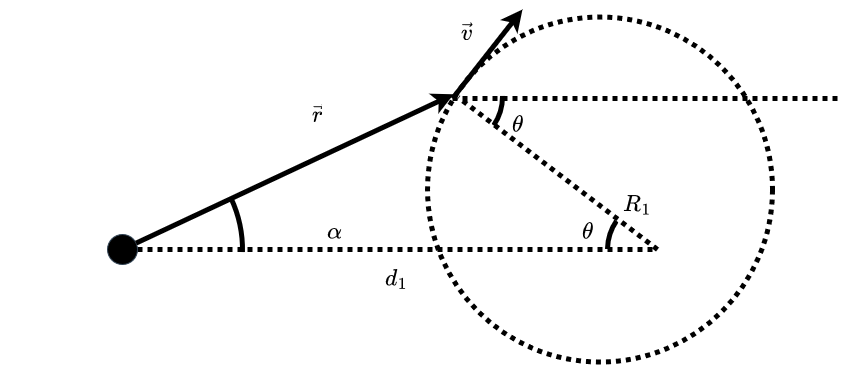
\includegraphics[width=\linewidth]{../diagrams/fern-v3-single-arm-angles-diagram.png}   
	 	\caption{Components of angular momentum integration.}
	 	\label{fig:one-arm-integral-angles}
 	\end{figure}

	Continuing...
	\begin{align}
		sin(\phi(\theta)) &= sin(\frac{\pi}{2}-(\theta+\alpha(\theta)))
	\end{align}

	To simplify...
	\begin{align}
		sin(\phi(\theta)) &= cos(\theta + \alpha(\theta)) \\
		 &= cos(\theta)cos(\alpha(\theta)) - sin(\theta)sin(\alpha(\theta)) \\
		 &= cos(\theta)cos(sin^{-1}(\frac{R_1sin(\theta)}{|\vec{r}(\theta)|})) - sin(\theta)sin(sin^{-1}(\frac{R_1sin(\theta)}{|\vec{r}(\theta)|})) \\
		 &= cos(\theta)\sqrt{1-\frac{R_1^2sin^2(\theta)}{|\vec{r}(\theta)|^2}} - \frac{R_1}{|\vec{r}(\theta)|}sin^2(\theta) \\
		 &= cos(\theta)\sqrt{\frac{|\vec{r}(\theta)|^2 - R_1^2sin^2(\theta)}{|\vec{r}(\theta)|^2}} - \frac{R_1}{|\vec{r}(\theta)|}sin^2(\theta) \\
		 &= cos(\theta)\sqrt{\frac{R_1^2+d_1^2-2R_1d_1cos(\theta)- R_1^2sin^2(\theta)}{|\vec{r}(\theta)|^2}} - \frac{R_1}{|\vec{r}(\theta)|}sin^2(\theta) \\
		 &= cos(\theta)\sqrt{\frac{R_1^2(1-sin^2(\theta))+d_1^2-2R_1d_1cos(\theta)}{|\vec{r}(\theta)|^2}} - \frac{R_1}{|\vec{r}(\theta)|}sin^2(\theta) \\
		 &= cos(\theta)\sqrt{\frac{R_1^2cos^2(\theta)+d_1^2-2R_1d_1cos(\theta)}{|\vec{r}(\theta)|^2}} - \frac{R_1}{|\vec{r}(\theta)|}sin^2(\theta) \\
		 &= cos(\theta)\sqrt{\frac{(R_1cos(\theta) - d_1)^2}{|\vec{r}(\theta)|^2}} - \frac{R_1}{|\vec{r}(\theta)|}sin^2(\theta) \\
		 &= \frac{d_1cos(\theta) - R_1cos^2(\theta) - R_1sin^2(\theta)}{|\vec{r}(\theta)|} \\
		 &= \frac{d_1cos(\theta) - R_1(cos^2(\theta) + sin^2(\theta))}{|\vec{r}(\theta)|} \\
		 &= \frac{d_1cos(\theta) - R_1}{|\vec{r}(\theta)|}
	\end{align}
	Recall...
	\begin{align}
		L &= \rho\int_0^{2\pi}|\vec{r}(\theta)||\vec{v}|sin(\phi(\theta))d\theta
	\end{align}

	Finally...
	\begin{align}
		L &=\rho\omega R_1\int_0^{2\pi}|\vec{r}(\theta)|\frac{d_1cos(\theta) - R_1}{|\vec{r}(\theta)|}d\theta \\
		 &= \rho\omega R_1\int_0^{2\pi}d_1cos(\theta) - R_1 d\theta \\
		 &= \rho\omega R_1^2 2\pi \\
		 &= \frac{m}{2\pi} \omega R_1^2 2\pi  \\
		 &= m \omega R_1^2
	\end{align}
	
\end{document}
